\documentclass[11pt]{article}

\usepackage[a4paper,margin=1in]{geometry}
\usepackage[T1]{fontenc}
\usepackage[utf8]{inputenc}
\usepackage{lmodern}
\usepackage{microtype}
\usepackage{amsmath,amssymb,amsthm,mathtools}
\usepackage{booktabs}
\usepackage{graphicx}
\usepackage{float}
\usepackage{placeins}
\usepackage{enumitem}
\usepackage[numbers,sort&compress]{natbib}
\usepackage{xcolor}
\usepackage{xurl}
\usepackage[colorlinks=true,linkcolor=blue!55!black,citecolor=blue!55!black,urlcolor=blue!55!black]{hyperref}
\usepackage[nameinlink,noabbrev]{cleveref}

\setlength{\parindent}{1.4em}
\setlength{\parskip}{0.15em}
\setlist{itemsep=0.25em,topsep=0.35em}

\newtheorem{theorem}{Theorem}[section]
\newtheorem{proposition}[theorem]{Proposition}
\newtheorem{lemma}[theorem]{Lemma}
\newtheorem{corollary}[theorem]{Corollary}
\theoremstyle{definition}
\newtheorem{definition}[theorem]{Definition}
\theoremstyle{remark}
\newtheorem{remark}[theorem]{Remark}

\newcommand{\R}{\mathbb R}
\newcommand{\C}{\mathbb C}
\newcommand{\N}{\mathbb N}
\newcommand{\uc}{u_{\mathrm c}}
\newcommand{\Id}{\mathrm I}
\newcommand{\cW}{\mathcal W}
\newcommand{\bW}{\mathbf W}
\newcommand{\cK}{\mathcal K}
\newcommand{\cP}{\mathcal P}
\newcommand{\cG}{\mathcal G}
\newcommand{\cond}{\operatorname{cond}_2}
\newcommand{\spec}{\operatorname{spec}}

\title{\textbf{Time-Ordered Boundary Monodromy}\
\textbf{at a Quadratic Band-Merging Map:}\\[0.35em]
\large Exact Geometric Cycle Determinants and a Nonuniform-Conditioning Barrier}
\author{Liang Wang\\
\small School of Artificial Intelligence and Automation,\\[-0.2em]
\small Huazhong University of Science and Technology, Wuhan 430074, P.R. China\\
\small \texttt{wangliang.f@gmail.com}}
\date{July 2026}

\begin{document}

\maketitle

\begin{abstract}
At the first algebraic band-merging parameter of
$f_u(x)=1-u x^2$, the parity-extracted deterministic bulk determinant has
the exact edge factor $(1-z^2/\lambda)^{-1}$.  Its canonical degree-$N$
finite section is
$\Pi_N(z^2/\lambda)=1+z^2/\lambda+\cdots+(z^2/\lambda)^N$,
whose reciprocal zeros form the roots-of-unity cloud observed for the
Gaussian Markov operator.  The preceding endpoint-rank theorem supplied the
correct half-logarithmic number of directions but did not supply their time
ordering.  We construct the missing deterministic time-ordered model and
identify a new obstruction to transferring it to the noisy operator.

Let $S=f^2$, and let $p_{2k}$ be the primitive boundary cycle coded by
$CA(CB)^{k-1}$.  We first show that its own $S$-orbit is an exact length-$k$
closed chain.  This chain, rather than the collection of endpoint points from
different periods, is the dynamically invariant object.  We then prove the
new critical-return multiplier law
\[
 (S^k)'(p_{2k})=-C_M\lambda^k(1+o(1)),
 \qquad C_M>0.
\]
The exponent is only $k$, although $S'(r)=\lambda^2$: the final return passes
within $O(\lambda^{-k})$ of the quadratic critical point and cancels one
power of the repelling expansion.

Weighting the ordered chain by $\omega_{k,j}=|S'(x_{k,j})|^{-1}$ gives a
finite cyclic transfer matrix $W_k$.  Put
$\rho_k=|(S^k)'(p_{2k})|^{-1/k}$.  Every choice of its individual weights is
removed by an exact diagonal similarity, and after the canonical bipartite
one-step lift one obtains
\[
 \boxed{
 \frac{\det(\Id-z\mathbf W_k)}{1-\rho_kz^2}
 =\Pi_{k-1}(\rho_kz^2).}
\]
Consequently the edge-deflated reciprocal cloud has exact phases
$\pm j\pi/k$ and radius
\[
 \sqrt{\rho_k}
 =\lambda^{-1/2}
 \exp\!\left[-\frac{\log C_M}{2k}+o(k^{-1})\right].
\]
This corrects an earlier ``finite unilateral shift'' description: a bare
finite unilateral shift is nilpotent and has determinant one; the geometric
polynomial requires a cyclic return followed by edge deflation.

The correction is not cosmetic.  The canonical diagonal balance has
condition number at least $c\lambda^k$, and the Euclidean eigenvalue
condition numbers are at least $c\lambda^k/k$.  At the endpoint-rank scale
$k=\log(1/\sigma)/(2\log\lambda)+O(1)$ these bounds become
$\Omega(\sigma^{-1/2})$ and
$\Omega(\sigma^{-1/2}/\log(1/\sigma))$.  Thus a uniformly conditioned
Euclidean Feshbach identification is unavailable for the unrenormalized
orbit basis; an adapted norm or structured Grushin normalization is needed.

High-precision computations give
$C_M=1.946342905200967\ldots$.  With the integer selected independently from
the preceding endpoint-row calculation, the resulting finite-$k$ radii are
closer than the limiting radius to every archived cloud mean.  These spectral
comparisons are ordinary floating-point diagnostics.  We do not claim that
$W_k$ is already a Feshbach block of the noisy Markov operator.
\end{abstract}

\noindent\textbf{Keywords:} transfer operator; weighted cyclic shift;
periodic monodromy; Gaussian perturbation; resonance cloud; Grushin problem;
non-normal spectrum; quadratic map.

\medskip
\noindent\textbf{MSC 2020:} 37E05; 37D25; 37C30; 47A10; 47A55; 65P30.

\section{Introduction}
\label{sec:introduction}

The small-noise spectral problem at a band-merging map has now separated into
three scales.  The peripheral negative resonance is governed by a coupled
critical-value boundary layer and satisfies a square-root splitting law
\citep{WangBoundaryLayer2026}.  After that mode and the Perron mode are
removed, the deterministic bulk determinant has the exact factorization
\begin{equation}\label{eq:intro-pole}
 \widehat D_{0,\mathrm{bulk},2}(z)
 =\frac{\cG(z)}{1-z^2/\lambda},
 \qquad \cG(z)\ne0\quad (|z|<\lambda),
\end{equation}
so locally uniform convergence of the entire noisy determinants through
$z=\pm\sqrt\lambda$ is impossible
\citep{WangBulkScattering2026}.  Finally, the endpoint Gaussian row family
has an intrinsic threshold rank
\begin{equation}\label{eq:intro-rank}
 N_\sigma^{\mathrm{row}}
 =\frac{\log(1/\sigma)}{2\log\lambda}+O(1),
\end{equation}
both for Hellinger fingerprints and for normalized linear kernel rows
\citep{WangEndpointRank2026}.

The missing arrow is dynamical.  Singular values count stable row directions,
but they do not specify how the transfer operator moves those directions.
The archived noisy spectra suggest the geometric section
\begin{equation}\label{eq:intro-section}
 \Pi_N(q)=1+q+\cdots+q^N,
 \qquad q=z^2/\lambda,
\end{equation}
because its reciprocal zeros have radius $\lambda^{-1/2}$ and phases
$\pm j\pi/(N+1)$.  The previous route map described this as the
characteristic polynomial of a finite unilateral shift.  Literally, that
statement is false: if $U_N$ is the ordinary finite unilateral shift, then
$U_N^N=0$ and
\begin{equation}\label{eq:nilpotent-warning}
 \det(\Id-qU_N)=1.
\end{equation}
The polynomial $\Pi_N$ is instead the determinant of a cyclic shift after
one distinguished eigenvalue has been removed:
\begin{equation}\label{eq:cyclic-preview}
 \frac{\det(\Id-qC_{N+1})}{1-q}
 =\frac{1-q^{N+1}}{1-q}=\Pi_N(q).
\end{equation}
This paper replaces the inaccurate unilateral wording by an exact dynamical
cyclic return.

The correction does not alter the pole theorem
\eqref{eq:intro-pole}, the algebraic finite section
\eqref{eq:intro-section}, or the archived noisy cloud.  It changes the
operator mechanism that must be proved.  A one-way chain is insufficient;
one needs a closed time-ordered chain, a distinguished edge channel to
deflate, and quantitative control of the basis that balances its weights.

\subsection*{Main results and logical status}

Let $p_{2k}$ denote the boundary point constructed from the inverse word
$CA(CB)^{k-1}$, and let $S=f^2$.  The paper establishes the following.

\begin{enumerate}[label=\textbf{M\arabic*.},leftmargin=3.2em]
 \item \textbf{Exact time order.}
 The $S$-orbit of $p_{2k}$ is an explicit cyclic chain of length $k$.
 In contrast, the endpoint dictionary
 $\{p_{2k}:k\ge1\}$ is not forward invariant: every $p_{2k}$ with $k\ge2$
 moves a fixed positive distance away from the entire dictionary in one
 component step.

 \item \textbf{Boundary multiplier theorem.}
 If $M_k=(S^k)'(p_{2k})$, then
 \begin{equation}\label{eq:intro-multiplier}
  M_k=-C_M\lambda^k(1+o(1)),
  \qquad C_M>0.
 \end{equation}
 This is an analytic theorem.  The displayed decimal for $C_M$ later in the
 paper is a high-precision computation, not an interval enclosure.

 \item \textbf{Exact geometric determinant.}
 The inverse-Jacobian weighted cyclic chain has an edge-deflated bipartite
 determinant exactly equal to
 \begin{equation}\label{eq:intro-exact-geometric}
  \Pi_{k-1}(\rho_kz^2),
  \qquad \rho_k=|M_k|^{-1/k}.
 \end{equation}
 Thus both the phase grid and the limiting radius follow from the same
 deterministic time ordering.

 \item \textbf{Conditioning barrier.}
 The diagonal similarity that balances the cycle has
 $\cond(D_k)\ge c\lambda^k$.  The ordinary Euclidean eigenvalue condition
 number has the lower bound $c\lambda^k/k$.  These are analytic statements;
 they rule out one particular uniformly conditioned reduction strategy, not
 every adapted-space construction.

 \item \textbf{Numerical comparison.}
 At the seven archived noises, finite-cycle radii selected from the independent
 Hellinger or linear row ranks are closer to the cloud means than the limiting
 value $\lambda^{-1/2}$.  This is reproducible floating-point evidence only.
 No equality between row rank, monodromy dimension, and Markov cloud degree is
 promoted to a theorem.
\end{enumerate}

The resulting logical chain is
\begin{equation}\label{eq:logical-chain}
 \boxed{
 \begin{gathered}
 \text{boundary word}
 \Longrightarrow
 \text{exact weighted cyclic monodromy}
 \Longrightarrow
 \Pi_{k-1}(\rho_kz^2),\\
 \text{noisy Markov Feshbach block}
 \quad\Longrightarrow?\quad
 \text{that monodromy in an adapted norm}.
 \end{gathered}}
\end{equation}
The upper line is proved here.  The lower arrow remains the next operator
problem.

\section{The boundary word and component dynamics}
\label{sec:setup}

Let $\uc$ be the root in $(1,2)$ of
\begin{equation}\label{eq:cubic}
 u^3-2u^2+2u-2=0,
\end{equation}
and put
\begin{equation}\label{eq:constants}
 f(x)=1-\uc x^2,
 \qquad r=\uc-1,
 \qquad \lambda=2\uc r.
\end{equation}
Then
\begin{equation}\label{eq:critical-orbit}
 0\longmapsto1\longmapsto-r\longmapsto r\longmapsto r
\end{equation}
and
\begin{equation}\label{eq:numerical-constants}
 \uc=1.543689012692076\ldots,
 \quad r=0.543689012692076\ldots,
 \quad \lambda=1.678573510428322\ldots.
\end{equation}
Write $S=f^2$.  The fixed point $r$ has
\begin{equation}\label{eq:S-derivative-r}
 S'(r)=\lambda^2.
\end{equation}

For $y\in[-r,1]$, define the two inverse branches
\begin{equation}\label{eq:inverse-branches}
 g_+(y)=\sqrt{\frac{1-y}{\uc}},
 \qquad
 g_-(y)=-\sqrt{\frac{1-y}{\uc}},
\end{equation}
and the two inverse component branches
\begin{equation}\label{eq:hq}
 h=g_+\circ g_+,
 \qquad q=g_+\circ g_-.
\end{equation}
On their corresponding branches,
\begin{equation}\label{eq:inverse-identities}
 S\circ h=\Id,
 \qquad S\circ q=\Id.
\end{equation}
At $r$,
\begin{equation}\label{eq:hq-data}
 h(r)=r,
 \quad h'(r)=a:=\lambda^{-2},
 \quad q(r)=1,
 \quad q'(r)=-\frac1{2\uc\lambda}.
\end{equation}

For $k\ge1$, the word $CA(CB)^{k-1}$ has inverse composition
\begin{equation}\label{eq:Gk}
 G_k=q\circ h^{k-1}.
\end{equation}
Its unique fixed point is denoted by
\begin{equation}\label{eq:pk-definition}
 p_k:=p_{2k}=G_k(p_k),
 \qquad \delta_k=1-p_k.
\end{equation}
The subscript $k$ will always mean component time; the physical period is
$2k$.  The boundary-crowding theorem gives
\begin{equation}\label{eq:clearance-law}
 \delta_k=C_{\mathrm b}a^k(1+o(1))
 =C_{\mathrm b}\lambda^{-2k}(1+o(1)),
 \qquad C_{\mathrm b}>0
\end{equation}
\citep{WangLongCycle2026,WangEndpointRank2026}.

The proof below uses the Koenigs coordinate $\psi$ of $h$ at $r$,
normalized by
\begin{equation}\label{eq:koenigs}
 \psi(h(x))=a\psi(x),
 \qquad \psi(r)=0,
 \qquad \psi'(r)=1.
\end{equation}
The coordinate is analytic near $r$ and extends along the real attracting
basin.  Although $h'$ is singular at $1$, the point
\begin{equation}\label{eq:b-definition}
 b:=h(1)=\uc^{-1/2}
\end{equation}
is interior, so $0<\psi'(b)<\infty$.

\section{The exact time-ordered return chain}
\label{sec:time-order}

The endpoint points $p_k$ come from different periodic orbits.  Time
evolution does not move from $p_k$ to $p_{k-1}$.  The correct chain lies
inside one boundary orbit.

\begin{theorem}[Exact boundary-word time order]
\label{thm:time-order}
For $k\ge1$, define
\begin{equation}\label{eq:ordered-points}
 x_{k,0}=p_k,
 \qquad
 x_{k,j}=h^{k-j}(p_k),
 \quad 1\le j\le k-1.
\end{equation}
Then these are the $k$ distinct points of the $S$-cycle of $p_k$, in forward
time order:
\begin{equation}\label{eq:cyclic-time-order}
 S(x_{k,j})=x_{k,j+1}\quad(0\le j<k-1),
 \qquad
 S(x_{k,k-1})=x_{k,0}.
\end{equation}
\end{theorem}

\begin{proof}
The fixed-point identity in \eqref{eq:pk-definition} is
$p_k=q(h^{k-1}(p_k))$.  Applying $S\circ q=\Id$ gives
\[
 S(p_k)=h^{k-1}(p_k)=x_{k,1}.
\]
For $1\le j<k-1$, apply $S\circ h=\Id$ to obtain
\[
 S(h^{k-j}(p_k))=h^{k-j-1}(p_k)=x_{k,j+1}.
\]
The same identity at the final point gives $S(h(p_k))=p_k$.  Distinctness
follows from primitivity of $CA(CB)^{k-1}$.
\end{proof}

The first internal point lies in the repelling-boundary layer.  Its scale is
the same as the endpoint clearance.

\begin{corollary}[Endpoint-to-repelling scale bridge]
\label{cor:scale-bridge}
As $k\to\infty$,
\begin{equation}\label{eq:scale-bridge}
 x_{k,1}-r
 =\frac{\delta_k}{-q'(r)}(1+o(1))
 =2\uc\lambda\,\delta_k(1+o(1)).
\end{equation}
In particular, the endpoint ladder across different periods and the first
internal levels of the ordered cycles have the same
$\lambda^{-2k}$ resolution clock.
\end{corollary}

\begin{proof}
By \eqref{eq:ordered-points} and \eqref{eq:pk-definition},
$p_k=q(x_{k,1})$.  Since $x_{k,1}\to r$ and $q(r)=1$, Taylor expansion gives
\[
 \delta_k=1-q(x_{k,1})
 =-q'(r)(x_{k,1}-r)(1+o(1)).
\]
Insert \eqref{eq:hq-data}.
\end{proof}

\subsection{Why the cross-period endpoint dictionary cannot be the shift}

The failure of direct endpoint time ordering is separated from the later
conditioning issue.

\begin{proposition}[Fixed gap after one component step]
\label{prop:endpoint-gap}
The points $p_k$ increase with $k$.  For every $k\ge2$,
\begin{equation}\label{eq:endpoint-gap}
 S(p_k)<b=h(1)<p_1\le p_j
 \qquad(j\ge1).
\end{equation}
Thus $S(p_k)$ is separated from the entire cross-period endpoint dictionary
by the fixed gap
\begin{equation}\label{eq:gap-constant}
 d_*=p_1-b=0.096158898694365\ldots>0.
\end{equation}
\end{proposition}

\begin{proof}
On $(r,1)$, $h$ is increasing and $h(x)<x$, while $q$ is decreasing.  Hence
$G_{k+1}(x)=q(h^k(x))>q(h^{k-1}(x))=G_k(x)$.  Each $G_k$ is decreasing, so
the unique zero of $G_k(x)-x$ moves to the right: $p_{k+1}>p_k$.
Moreover, $p_1<1$ and the explicit formula for $q$ gives
\[
 p_1=q(p_1)
 =\sqrt{\frac{1+\sqrt{(1-p_1)/\uc}}{\uc}}
 >\uc^{-1/2}=b.
\]

For $k\ge2$, \cref{thm:time-order} and monotonicity of $h$ give
\[
 S(p_k)=h^{k-1}(p_k)\le h(p_k)<h(1)=b.
\]
The monotonicity of $p_j$ gives the remaining inequalities.  The decimal is
a high-precision evaluation of $p_1-b$.
\end{proof}

\begin{remark}[Consequence for a localized compression]
\label{rem:localized-compression}
A family of packets concentrated at the points $p_k$ cannot be permuted by
one application of the two-step dynamics: all nontrivial packets move into a
neighborhood of $[r,b]$, a fixed distance from their original centers.
Consequently the RH-16 endpoint row dictionary can supply a dimension count,
but it cannot by itself be the time-ordered basis.  Any noisy Feshbach block
must include the internal chain \eqref{eq:ordered-points} and the coupling
between the endpoint and repelling-boundary layers.
\end{remark}

\section{A critical-return multiplier theorem}
\label{sec:multiplier}

Let
\begin{equation}\label{eq:Mk-definition}
 M_k=(S^k)'(p_k)
 =\prod_{j=0}^{k-1}S'(x_{k,j}).
\end{equation}
If every factor were asymptotic to $S'(r)=\lambda^2$, one might expect
$|M_k|$ to grow like $\lambda^{2k}$.  The final factor is instead
exponentially small because $x_{k,k-1}=h(p_k)$ maps through a point close to
the critical point.

\begin{lemma}[Endpoint derivative of the inverse branch]
\label{lem:h-endpoint-derivative}
As $\delta\downarrow0$,
\begin{equation}\label{eq:h-endpoint-derivative}
 h'(1-\delta)
 =\frac1{4\uc\sqrt\delta}(1+O(\sqrt\delta)).
\end{equation}
Consequently
\begin{equation}\label{eq:hpk-derivative}
 h'(p_k)
 =\frac{\lambda^k}{4\uc\sqrt{C_{\mathrm b}}}(1+o(1)).
\end{equation}
\end{lemma}

\begin{proof}
Differentiating $h=g_+\circ g_+$ gives
\begin{equation}\label{eq:hprime-exact}
 h'(x)=\frac1{4\uc^2h(x)g_+(x)}.
\end{equation}
For $x=1-\delta$,
$g_+(x)=\sqrt{\delta/\uc}$ and
$h(x)=\uc^{-1/2}+O(\sqrt\delta)$.  Substitution proves
\eqref{eq:h-endpoint-derivative}.  Apply
\eqref{eq:clearance-law} and $a^{-k/2}=\lambda^k$ to obtain
\eqref{eq:hpk-derivative}.
\end{proof}

\begin{theorem}[Critical-return boundary multiplier law]
\label{thm:multiplier-law}
There is a constant $C_M>0$ such that
\begin{equation}\label{eq:multiplier-law}
 \boxed{
 M_k=-C_M\lambda^k(1+o(1)).}
\end{equation}
With $b=\uc^{-1/2}$ and the normalization
\eqref{eq:koenigs}, the constant is
\begin{equation}\label{eq:CM-formula}
 C_M
 =\frac{4\uc\sqrt{C_{\mathrm b}}}
 {|q'(r)|\psi'(b)\lambda^4}.
\end{equation}
\end{theorem}

\begin{proof}
The map $G_k=q\circ h^{k-1}$ is the inverse branch of $S^k$ that fixes
$p_k$.  Therefore
\begin{equation}\label{eq:inverse-multiplier}
 M_k=\frac1{G_k'(p_k)}.
\end{equation}
Separate the singular first derivative of $h^{k-1}$:
\begin{equation}\label{eq:split-h-derivative}
 (h^{k-1})'(p_k)
 =h'(p_k)(h^{k-2})'(h(p_k)).
\end{equation}
Differentiating the Koenigs identity
$\psi(h^n(x))=a^n\psi(x)$ gives
\begin{equation}\label{eq:koenigs-derivative}
 (h^n)'(x)
 =a^n\frac{\psi'(x)}{\psi'(h^n(x))}.
\end{equation}
Use this with $n=k-2$ and $x=h(p_k)$.  Since
$h(p_k)\to b$, $h^{k-1}(p_k)\to r$, and $\psi'(r)=1$,
\begin{equation}\label{eq:interior-h-derivative}
 (h^{k-2})'(h(p_k))
 =a^{k-2}\psi'(b)(1+o(1)).
\end{equation}
Combining \cref{lem:h-endpoint-derivative} with
\eqref{eq:interior-h-derivative} gives
\begin{align}
 (h^{k-1})'(p_k)
 &=\frac{\psi'(b)}{4\uc\sqrt{C_{\mathrm b}}}
 a^{k-2-k/2}(1+o(1))\notag\\
 &=\frac{\psi'(b)\lambda^4}{4\uc\sqrt{C_{\mathrm b}}}
 \lambda^{-k}(1+o(1)).
 \label{eq:h-full-asymptotic}
\end{align}
Moreover,
$q'(h^{k-1}(p_k))=q'(r)(1+o(1))$.  Hence
\[
 G_k'(p_k)
 =q'(r)\frac{\psi'(b)\lambda^4}
 {4\uc\sqrt{C_{\mathrm b}}}
 \lambda^{-k}(1+o(1)).
\]
The derivative is negative.  Inverting it proves
\eqref{eq:multiplier-law} and \eqref{eq:CM-formula}.
\end{proof}

\begin{remark}[Where the missing power goes]
\label{rem:critical-cancellation}
The final point of the ordered chain is $x_{k,k-1}=h(p_k)$.  From
$S\circ h=\Id$,
\begin{equation}\label{eq:final-derivative}
 S'(h(p_k))=\frac1{h'(p_k)}
 =4\uc\sqrt{C_{\mathrm b}}\,\lambda^{-k}(1+o(1)).
\end{equation}
The other $k-1$ factors collectively carry the repelling expansion.  The
single critical return \eqref{eq:final-derivative} removes one exponential
power, leaving $|M_k|\asymp\lambda^k$ rather than
$\lambda^{2k}$.
\end{remark}

\section{Weighted cyclic monodromy and the geometric determinant}
\label{sec:cycle-determinant}

The physical flat trace is associated with the inverse-Jacobian stability
channel \citep{Baladi2000}.  Along the ordered cycle, define
\begin{equation}\label{eq:weights}
 \omega_{k,j}=\frac1{|S'(x_{k,j})|},
 \qquad 0\le j\le k-1,
\end{equation}
and let $W_k$ act on the standard basis of $\C^k$ by
\begin{equation}\label{eq:weighted-shift}
 W_ke_j=\omega_{k,j}e_{j+1\pmod k}.
\end{equation}
Its total weight is
\begin{equation}\label{eq:weight-product}
 \prod_{j=0}^{k-1}\omega_{k,j}=|M_k|^{-1}.
\end{equation}
Put
\begin{equation}\label{eq:rho-definition}
 \rho_k=|M_k|^{-1/k}.
\end{equation}

\begin{theorem}[Exact balancing and cyclic determinant]
\label{thm:weighted-cycle}
There is a positive diagonal matrix $D_k$ such that
\begin{equation}\label{eq:cycle-similarity}
 D_k^{-1}W_kD_k=\rho_kC_k,
\end{equation}
where $C_ke_j=e_{j+1\pmod k}$ is the unweighted cyclic shift.  Consequently
\begin{align}
 W_k^k&=\rho_k^k\Id,
 \label{eq:W-power}\\
 \spec(W_k)&=\{\rho_ke^{2\pi i\ell/k}:0\le\ell<k\},
 \label{eq:W-spectrum}\\
 \det(\Id-wW_k)&=1-(\rho_kw)^k.
 \label{eq:W-determinant}
\end{align}
\end{theorem}

\begin{proof}
Choose $d_{k,0}>0$ and define cyclically
\begin{equation}\label{eq:d-recurrence}
 d_{k,j+1}=\frac{\omega_{k,j}}{\rho_k}d_{k,j}.
\end{equation}
The closure condition at $j=k-1$ holds because
$\prod_j\omega_{k,j}=\rho_k^k$.  With
$D_k=\operatorname{diag}(d_{k,0},\ldots,d_{k,k-1})$, each balanced matrix
entry equals $\rho_k$, proving \eqref{eq:cycle-similarity}.  The remaining
claims are the elementary spectrum and determinant of $C_k$.
\end{proof}

The original map exchanges two components in one step.  The canonical
bipartite lift of the component matrix is
\begin{equation}\label{eq:bipartite-lift}
 \bW_k=
 \begin{pmatrix}
  0&\Id\\
  W_k&0
 \end{pmatrix}
 \quad\text{on }\C^k\oplus\C^k.
\end{equation}
Then
$\bW_k^2=\operatorname{diag}(W_k,W_k)$ and a Schur complement gives
\begin{equation}\label{eq:bipartite-determinant}
 \det(\Id-z\bW_k)
 =\det(\Id-z^2W_k)
 =1-(\rho_kz^2)^k.
\end{equation}

\begin{remark}[Algebraic normalization of the lift]
\label{rem:bipartite-normalization}
The choice of an identity in the upper-right block is a normalization, not a
claim about the individual one-step branch weights.  More generally, if
$A_kB_k$ and $B_kA_k$ are the two component return matrices, then
\[
 \det\!\begin{pmatrix}\Id&-zA_k\\-zB_k&\Id\end{pmatrix}
 =\det(\Id-z^2B_kA_k).
\]
Thus the determinant depends only on the two-step monodromy.  Identifying
the separate blocks with the noisy one-step dynamics remains part of the
Feshbach problem in \cref{sec:noisy-relation}.
\end{remark}

\begin{corollary}[Exact edge-deflated geometric section]
\label{cor:geometric-section}
After removing the distinguished real edge pair $\pm\sqrt{\rho_k}$,
\begin{equation}\label{eq:exact-geometric-section}
 \boxed{
 \frac{\det(\Id-z\bW_k)}{1-\rho_kz^2}
 =\Pi_{k-1}(\rho_kz^2).}
\end{equation}
The reciprocal resonances of the quotient are exactly
\begin{equation}\label{eq:finite-cloud}
 \mu_{k,j}^{\pm}
 =\sqrt{\rho_k}\exp\!\left(\pm\frac{ij\pi}{k}\right),
 \qquad 1\le j\le k-1.
\end{equation}
\end{corollary}

\begin{proof}
Divide \eqref{eq:bipartite-determinant} by $1-\rho_kz^2$ and use the finite
geometric identity.  The zeros of $\Pi_{k-1}(q)$ are the nontrivial $k$th
roots of unity.  Taking both square roots and then reciprocals gives
\eqref{eq:finite-cloud}.
\end{proof}

The radius now follows from the multiplier theorem.

\begin{corollary}[Finite-radius law]
\label{cor:radius-law}
As $k\to\infty$,
\begin{align}
 \rho_k
 &=\lambda^{-1}
 \exp\!\left[-\frac{\log C_M}{k}+o(k^{-1})\right],
 \label{eq:rho-law}\\
 r_k:=\sqrt{\rho_k}
 &=\lambda^{-1/2}
 \exp\!\left[-\frac{\log C_M}{2k}+o(k^{-1})\right].
 \label{eq:radius-law}
\end{align}
Thus \eqref{eq:exact-geometric-section} tends coefficientwise to the RH-15
section $\Pi_{k-1}(z^2/\lambda)$.
\end{corollary}

\begin{proof}
Take logarithms in
$\rho_k=|M_k|^{-1/k}$ and use
\cref{thm:multiplier-law}.  The second identity is its square root.
\end{proof}

\subsection{Cyclic return versus unilateral truncation}

The distinction can be summarized algebraically.  Let $U_k$ be the
nilpotent shift $U_ke_j=e_{j+1}$ for $j<k-1$ and $U_ke_{k-1}=0$.  Then
\begin{equation}\label{eq:unilateral-determinant}
 \det(\Id-qU_k)=1.
\end{equation}
The resolvent of $U_k$ contains a finite geometric sum,
\begin{equation}\label{eq:unilateral-resolvent}
 (\Id-qU_k)^{-1}
 =\Id+qU_k+\cdots+q^{k-1}U_k^{k-1},
\end{equation}
but that sum is a matrix element or transfer function, not its determinant.
Closing the final arrow turns $U_k$ into $C_k$; only then does edge deflation
produce $\Pi_{k-1}$.  The boundary word supplies precisely this closing
arrow through $S(x_{k,k-1})=x_{k,0}$.

\begin{remark}[What the edge pair means]
\label{rem:edge-pair}
The factor $1-\rho_kz^2$ in
\eqref{eq:exact-geometric-section} is the distinguished channel of the cycle
model.  It is not the Perron/parity pair $\pm1$ of the deterministic Markov
dynamics.  Rather, its limit is the formal edge pair
$\pm\lambda^{-1/2}$ associated with the pole
$(1-z^2/\lambda)^{-1}$.  The geometric cloud is the determinant left after
that edge channel is removed.
\end{remark}

\section{The nonuniform-conditioning barrier}
\label{sec:conditioning}

The spectrum in \eqref{eq:W-spectrum} depends only on the product of the
weights.  Perturbative stability depends on their distribution.  Here the
critical return puts an exponentially large inverse-Jacobian weight on one
edge of the cycle.

Normalize $D_k$ by an arbitrary positive scalar and let
\begin{equation}\label{eq:D-condition}
 \kappa_k=\cond(D_k)
 =\frac{\max_jd_{k,j}}{\min_jd_{k,j}}.
\end{equation}
The last recurrence in \eqref{eq:d-recurrence} gives
\begin{equation}\label{eq:last-d-ratio}
 \frac{d_{k,0}}{d_{k,k-1}}
 =\frac{\omega_{k,k-1}}{\rho_k}.
\end{equation}

\begin{theorem}[Exponential balancing barrier]
\label{thm:conditioning-barrier}
There are $c>0$ and $k_0$ such that
\begin{equation}\label{eq:condition-lower}
 \boxed{
 \kappa_k\ge c\lambda^k
 \qquad(k\ge k_0).}
\end{equation}
More precisely,
\begin{equation}\label{eq:last-weight-law}
 \omega_{k,k-1}
 =\frac{\lambda^k}{4\uc\sqrt{C_{\mathrm b}}}(1+o(1)),
\end{equation}
and therefore
\begin{equation}\label{eq:ratio-asymptotic}
 \frac{d_{k,0}}{d_{k,k-1}}
 =\frac{\lambda^{k+1}}{4\uc\sqrt{C_{\mathrm b}}}(1+o(1)).
\end{equation}
\end{theorem}

\begin{proof}
The final ordered point is $x_{k,k-1}=h(p_k)$.  Since $S\circ h=\Id$,
\[
 \omega_{k,k-1}
 =\frac1{|S'(h(p_k))|}=h'(p_k).
\]
Equation \eqref{eq:last-weight-law} is therefore
\eqref{eq:hpk-derivative}.  Combine it with
$\rho_k\to\lambda^{-1}$ in \eqref{eq:last-d-ratio}.  Since the condition
number dominates the ratio of any two diagonal entries,
\eqref{eq:condition-lower} follows.
\end{proof}

The same imbalance appears in the ordinary eigenvalue condition numbers.
Let $f_\ell$ be a unit Fourier eigenvector of $C_k$.  From
\eqref{eq:cycle-similarity}, right and left eigenvectors of $W_k$ may be
chosen as $D_kf_\ell$ and $D_k^{-1}f_\ell$.  Their common Euclidean
eigenvalue condition number is
\begin{equation}\label{eq:eigenvalue-condition-exact}
 \chi_k
 =\frac{\|d_k\|_2\|d_k^{-1}\|_2}{k},
\end{equation}
where $d_k=(d_{k,0},\ldots,d_{k,k-1})$ and the inverse is componentwise.

\begin{corollary}[Eigenvalue sensitivity at the noise clock]
\label{cor:eigenvalue-conditioning}
For all sufficiently large $k$,
\begin{equation}\label{eq:eigen-condition-lower}
 \chi_k\ge\frac{\kappa_k}{k}
 \ge\frac{c\lambda^k}{k}.
\end{equation}
If
\begin{equation}\label{eq:noise-selected-k}
 k_\sigma
 =\frac{\log(1/\sigma)}{2\log\lambda}+O(1),
\end{equation}
then
\begin{align}
 \kappa_{k_\sigma}&=\Omega(\sigma^{-1/2}),
 \label{eq:condition-noise}\\
 \chi_{k_\sigma}
 &=\Omega\!\left(
 \frac{\sigma^{-1/2}}{\log(1/\sigma)}\right).
 \label{eq:eigen-condition-noise}
\end{align}
\end{corollary}

\begin{proof}
The two sums in \eqref{eq:eigenvalue-condition-exact} contain respectively
$\max_jd_{k,j}$ and $(\min_jd_{k,j})^{-1}$, proving the first inequality.
Equation \eqref{eq:noise-selected-k} gives
$\lambda^{k_\sigma}=\Theta(\sigma^{-1/2})$ and
$k_\sigma=\Theta(\log(1/\sigma))$.
\end{proof}

\begin{remark}[Interpretation, not an impossibility theorem]
\label{rem:not-impossibility}
The usual Bauer--Fike estimate would multiply a Euclidean operator-norm
remainder by an exponentially growing eigenvector condition number
\citep{Kato1995,TrefethenEmbree2005}.  Therefore a remainder merely small on
the $k^{-1}$ phase-spacing scale is not enough for this unbalanced basis.
This does not prove that the noisy cloud is unstable.  The perturbation is
structured, the Gaussian row Gram matrix is nontrivial, and an adapted
anisotropic norm can absorb part of the diagonal balance.  The theorem says
that uniform Euclidean pre- and post-conditioners cannot be assumed for the
raw orbit packets.
\end{remark}

\section{Relation to the noisy Gaussian operator}
\label{sec:noisy-relation}

For $\sigma>0$, let $\cK_\sigma$ be the row-normalized folded Gaussian
Markov operator on $[0,1]$ used in the preceding papers.  It is compact and
strongly positive, with Perron eigenvalue one and a simple negative parity
resonance.  After those two modes are removed, its bulk spectrum contains
the cloud compared below.

The matrix $W_k$ is not defined by projecting $\cK_\sigma^2$ onto computed
eigenvectors.  It is a deterministic first-stability-channel monodromy built
from an explicit periodic word.  This independence makes the phase theorem
noncircular, but it also leaves a genuine proof obligation.

\subsection{What has now been proved}

The following parts of the proposed shift mechanism are exact.

\begin{enumerate}[label=(\roman*),leftmargin=2.5em]
 \item The half-logarithmic row count has the same geometric scale as the
 first internal point of the time-ordered boundary cycle, by
 \cref{cor:scale-bridge}.
 \item The relevant time ordering is cyclic and is supplied by one primitive
 boundary orbit, by \cref{thm:time-order}.
 \item The inverse-Jacobian stability channel of that orbit gives the exact
 polynomial $\Pi_{k-1}(\rho_kz^2)$, by
 \cref{cor:geometric-section}.
 \item The limiting radius and its first $1/k$ correction follow from a new
 multiplier theorem, not from fitting the noisy cloud.
\end{enumerate}

\subsection{What has not been proved}

No theorem in this paper asserts
\begin{equation}\label{eq:not-feshbach}
 \text{Feshbach block of }\cK_\sigma
 \simeq \bW_{k_\sigma}.
\end{equation}
In particular, we do not prove equality among
\begin{equation}\label{eq:three-integers}
 N_\sigma^{\mathrm{Hellinger}},
 \qquad N_\sigma^{\mathrm{linear}},
 \qquad N_\sigma^{\mathrm{cloud}}.
\end{equation}
All three obey, or numerically follow, the same leading clock, but their
bounded staircase phases need not agree at finite noise.

The cross-period endpoint basis cannot fix this problem: by
\cref{prop:endpoint-gap}, its direct two-step compression misses the ordered
chain.  Conversely, the raw orbit basis has the exponential conditioning in
\cref{thm:conditioning-barrier}.  These two facts narrow the next
construction considerably.

\subsection{A corrected Grushin route}

A viable operator proof should contain four estimates.

\begin{enumerate}[label=\textbf{G\arabic*.},leftmargin=3.1em]
 \item \textbf{Paired boundary extraction.}
 Remove the RH-14 parity profile at $r$ and the critical-value endpoint layer
 at $1$ before forming the bulk Schur complement
 \citep{WangBoundaryLayer2026}.

 \item \textbf{Ordered transition space.}
 Build packets along the internal points $x_{k,j}$ of one boundary word,
 rather than using only the means $p_k$ from different words.  Use
 \cref{cor:scale-bridge} to compare the resulting approximation numbers with
 the RH-16 endpoint row operator.

 \item \textbf{Adapted balance.}
 Incorporate $D_k$ into the norm or into the entrance/exit maps of a Grushin
 problem.  Uniform conditioning in the unweighted Euclidean packet norm is
 contradicted by \eqref{eq:condition-noise}; the correct statement must be
 weighted or exploit the structured Gaussian remainder
 \citep{SjoestrandZworski2007}.

 \item \textbf{Residual normality.}
 After extracting the resulting cloud determinant, prove local bounds for the
 residual determinant on compact subsets of $|z|<\lambda$.  This remains
 necessary to identify the nonzero factor $\cG$ in
 \eqref{eq:intro-pole}.
\end{enumerate}

This route is more constrained than the previous ``unilateral shift plus a
small remainder'' formulation.  It specifies the closure edge, the edge
factor to deflate, the natural finite-radius correction, and the norm problem
that any perturbation argument must solve.

\section{High-precision and archived-spectrum audit}
\label{sec:numerics}

The analytic results above require no numerical hypothesis.  The computations
serve three narrower purposes: evaluate the constants, verify the exact
finite identities in an independent implementation, and compare the
parameter-free finite-$k$ radii with already archived noisy spectra.

\subsection{Method and reproducibility}

The fixed point of $G_k=q\circ h^{k-1}$ is evaluated by contraction with 130
decimal digits.  The multiplier is computed in two independent ways:
\begin{equation}\label{eq:numerical-multiplier-check}
 M_k=\prod_{j=0}^{k-1}S'(x_{k,j})
 =\frac1{G_k'(p_k)}.
\end{equation}
The test suite checks the equality, the exact cyclic time order, the diagonal
similarity, the bipartite determinant, the reciprocal roots, and the
conditioning bounds.  NumPy, mpmath, and Matplotlib provide the implementation
\citep{HarrisEtAl2020,Mpmath2026,Hunter2007}.

The calculation gives
\begin{equation}\label{eq:CM-numerical}
 C_M=1.946342905200967\ldots.
\end{equation}
The value of $|M_k|/\lambda^k$ is stable to the displayed digits by
$k=80$.  This is a multiprecision diagnostic, not a directed-rounding
certificate.

\begin{table}[H]
\centering
\small
\caption{Boundary-cycle multiplier, finite two-step radius, one-step radius,
and balancing.  Here $\rho_k=|M_k|^{-1/k}$ and
$r_k=\sqrt{\rho_k}$.}
\label{tab:multiplier}
\begin{tabular}{rrrrrr}
\toprule
$k$ & $\delta_k$ & $|M_k|/\lambda^k$ & $\rho_k$ & $r_k$
& $\cond(D_k)/\lambda^k$\\
\midrule
4  & $6.495\times10^{-3}$  & 1.8425567 & 0.5113337 & 0.7150760 & 0.511913\\
8  & $1.142\times10^{-4}$  & 1.9372562 & 0.5484806 & 0.7405947 & 0.440383\\
20 & $4.633\times10^{-10}$ & 1.9463261 & 0.5762340 & 0.7591008 & 0.414032\\
40 & $4.659\times10^{-19}$ & 1.9463429 & 0.5859076 & 0.7654460 & 0.407186\\
80 & $4.710\times10^{-37}$ & 1.9463429 & 0.5908053 & 0.7686386 & 0.403800\\
100& $4.736\times10^{-46}$ & 1.9463429 & 0.5917898 & 0.7692787 & 0.403138\\
\bottomrule
\end{tabular}
\end{table}

\Cref{fig:main-audit} displays the two asymptotic mechanisms.  The scaled
multiplier rapidly converges, while the balancing and eigenvalue condition
numbers grow exponentially.  The lower-right panel shows the exact $k=8$
time order: the endpoint first jumps into an exponentially thin layer above
$r$, then moves outward along the inverse-branch ladder before the critical
return closes the cycle.

\begin{figure}[H]
\centering
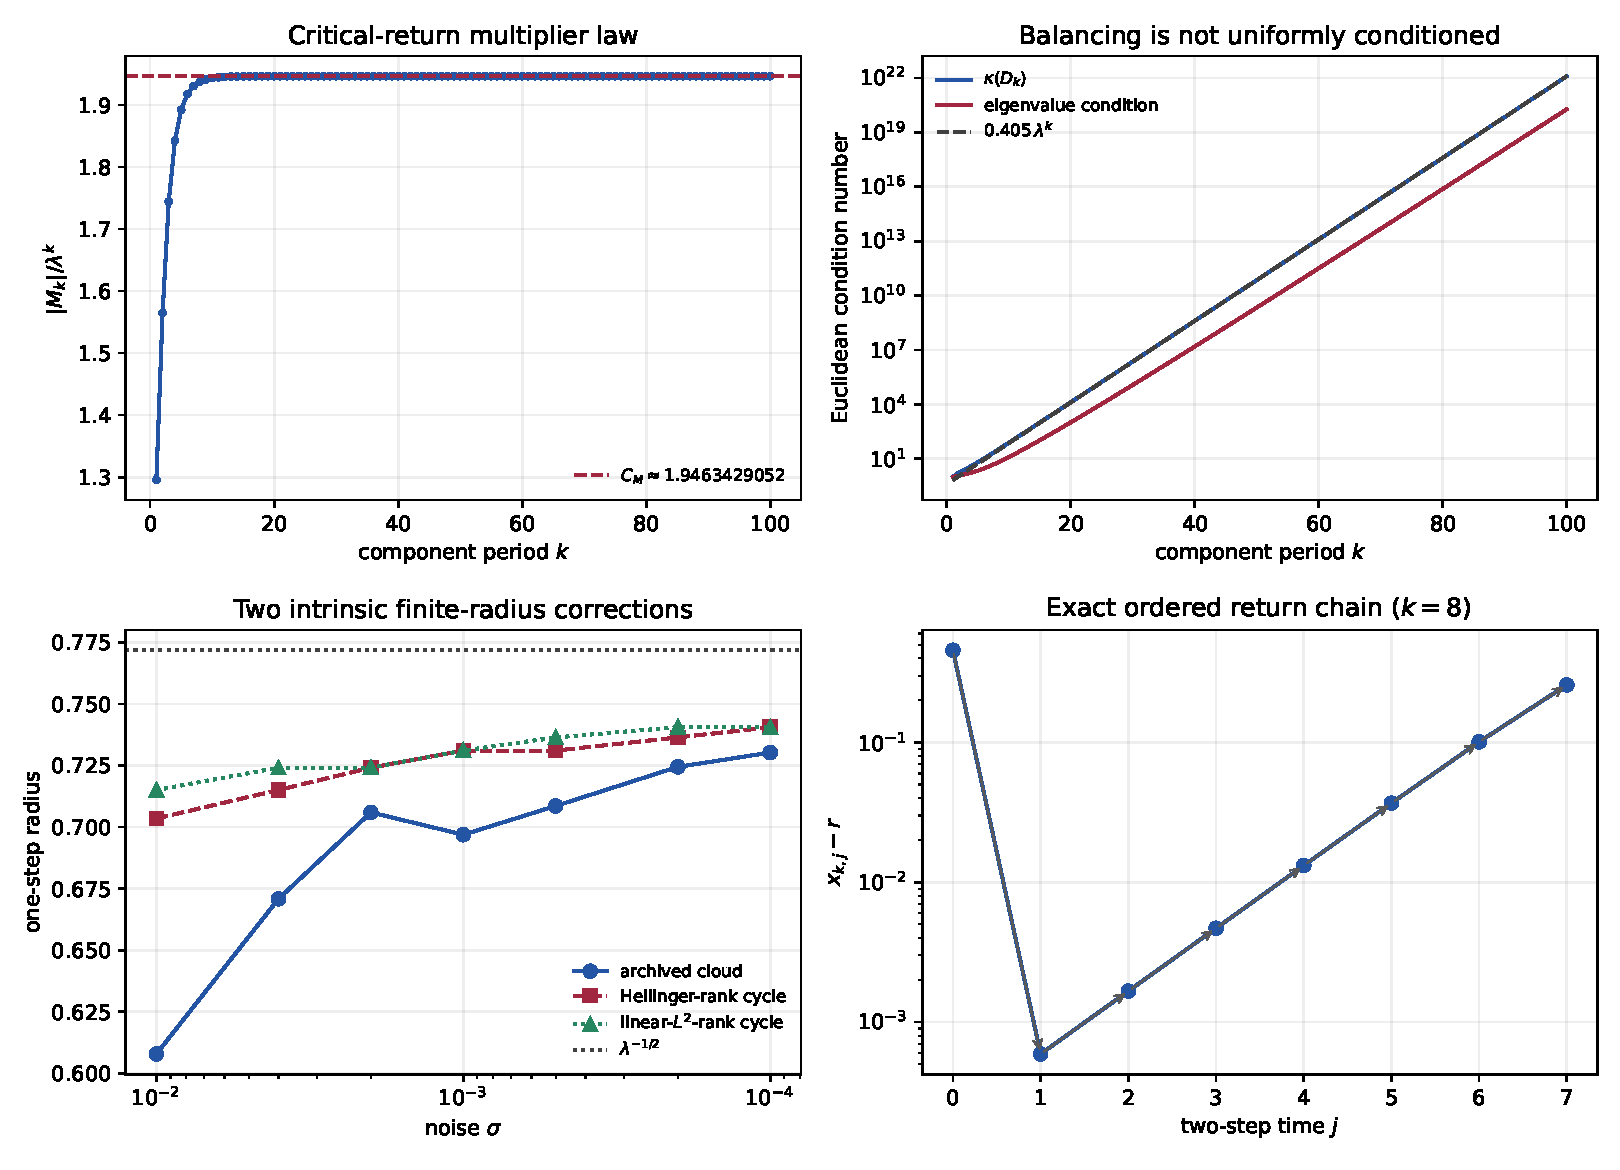
\includegraphics[width=\textwidth]{figures/time_ordered_boundary_monodromy.pdf}
\caption{Time-ordered boundary monodromy audit.  Top left: the multiplier law
$|M_k|\sim C_M\lambda^k$.  Top right: the canonical diagonal balance and the
ordinary eigenvalue condition number; the dashed line is a numerical
$\lambda^k$ reference.  Bottom left: archived noisy cloud radii and the two
finite-cycle predictions selected independently from the Hellinger and
linear-row ranks.  Bottom right: the exact two-step order of the $k=8$
boundary cycle, shown by distance from the repelling boundary $r$.}
\label{fig:main-audit}
\end{figure}

\subsection{Two intrinsic integer choices}

At each archived noise, we recompute the RH-16 half-energy counts
$s_j^2>1/2$ without reading any Markov eigenvalue.  The Hellinger and linear
row families have the same leading rank theorem but different bounded
staircase phases.  For each integer $N$, the cycle model uses $k=N+1$ and
predicts $r_k=|M_k|^{-1/(2k)}$.

\begin{table}[H]
\centering
\scriptsize
\caption{Intrinsic row degrees, archived cloud degree and mean radius, and
the two finite-cycle radius predictions.  The phase RMS is measured against
the common roots-of-unity grid.}
\label{tab:cloud-comparison}
\begin{tabular}{rrrrrrrr}
\toprule
$\sigma$ & $N_H$ & $N_L$ & $N_{\rm cloud}$ & $\bar r_{\rm cloud}$
& $r_{N_H+1}$ & $r_{N_L+1}$ & phase RMS\\
\midrule
$10^{-2}$        &2&3&3&0.607841&0.703501&0.715076&0.07933\\
$4\times10^{-3}$ &3&4&3&0.670849&0.715076&0.724152&0.07773\\
$2\times10^{-3}$ &4&4&4&0.705958&0.724152&0.724152&0.02431\\
$10^{-3}$        &5&5&5&0.696908&0.731090&0.731090&0.02184\\
$5\times10^{-4}$ &5&6&5&0.708586&0.731090&0.736423&0.04522\\
$2\times10^{-4}$ &6&7&6&0.724468&0.736423&0.740595&0.02636\\
$10^{-4}$        &7&7&7&0.730269&0.740595&0.740595&0.01124\\
\bottomrule
\end{tabular}
\end{table}

The Hellinger degree equals the archived cloud degree at six of seven points;
the linear-row degree does so at four of seven.  Every discrepancy is one.
This is consistent with, but does not sharpen, the analytic $O(1)$ rank
ambiguity.  It also prevents a claim that the transfer-relevant linear rank
has already identified the cloud count.

The finite-cycle correction is nevertheless robust.  The root-mean-square
radial errors over the seven points are
\begin{equation}\label{eq:radius-rms}
 \begin{array}{c|c}
 \text{radius model}&\text{RMS error}\\
 \hline
 \lambda^{-1/2}&0.0886635\\
 r_{N_H+1}&0.0436908\\
 r_{N_L+1}&0.0492538\\
 r_{N_{\rm cloud}+1}&0.0473750
 \end{array}
\end{equation}
The last line is conditional on the spectrally selected degree and is listed
only as a diagnostic.  The first two finite-cycle lines use no cloud
amplitude or phase fit.  All three finite choices improve the limiting radius
at every point in the table.

At $\sigma=10^{-4}$, both intrinsic ranks and the cloud selection give
$N=7$.  The deterministic $k=8$ cycle predicts
\begin{equation}\label{eq:smallest-radius-comparison}
 r_8=0.7405947445\ldots,
 \qquad
 \bar r_{\rm cloud}=0.7302687845\ldots,
 \qquad
 \lambda^{-1/2}=0.7718445063\ldots.
\end{equation}
The finite prediction has absolute error $0.01033$, compared with $0.04158$
for the limiting radius.

\begin{figure}[H]
\centering
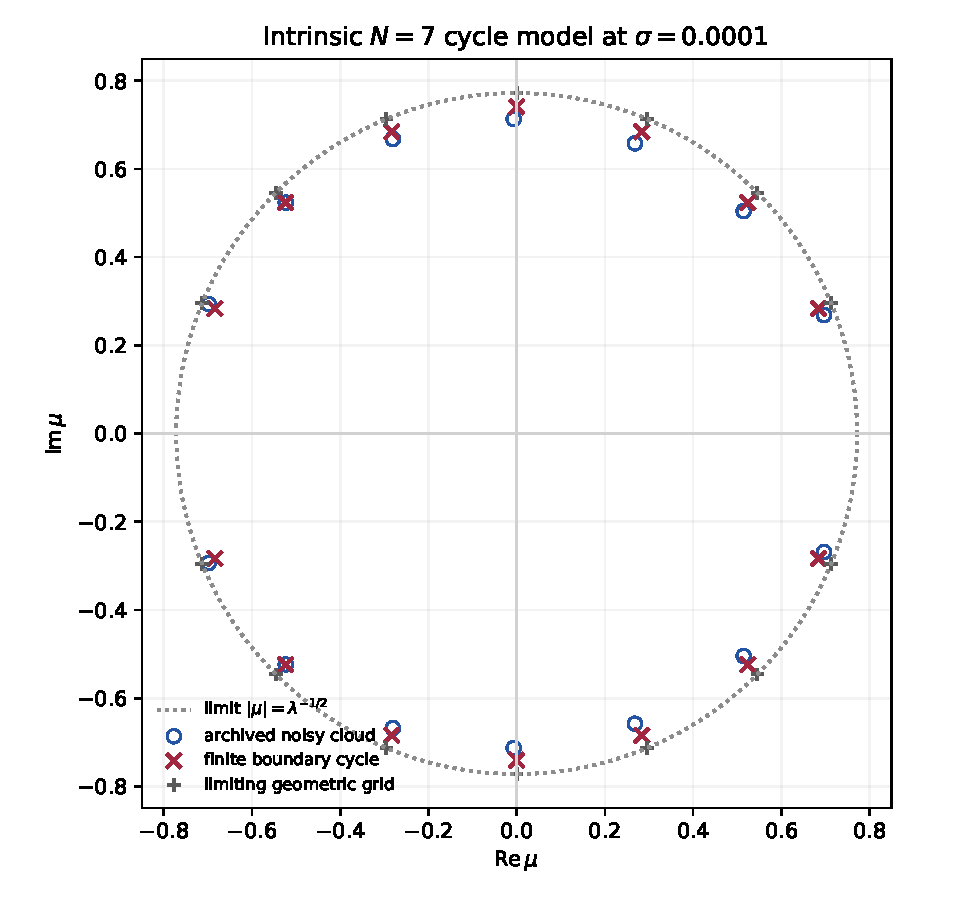
\includegraphics[width=0.77\textwidth]{figures/finite_cycle_cloud_overlay.pdf}
\caption{The smallest-noise cloud after the integer $N=7$ is selected
independently by both endpoint-row geometries.  Open circles are archived
Gaussian Markov resonances.  Crosses are the exact edge-deflated $k=8$
boundary-cycle monodromy, with no radial or phase fit.  Plus signs show the
same geometric phases at the limiting radius $\lambda^{-1/2}$.  The phase
agreement and finite-radius improvement are floating-point diagnostics, not
a Feshbach theorem.}
\label{fig:cloud-overlay}
\end{figure}

\subsection{Numerical status}

The boundary fixed points, multipliers and determinant identities are
computed with arbitrary-precision arithmetic.  The tests compare the product
and inverse-branch multipliers to more than 70 decimal places and verify the
matrix identities at double precision.  None of these calculations uses
interval arithmetic, so the decimal constants are not computer-assisted
theorems.

The noisy cloud means and phases are imported unchanged from the RH-15 sparse
ARPACK computation with up to $204800$ states.  The endpoint ranks are
recomputed from the exact RH-16 Gram kernels.  No noisy transfer matrix is
rebuilt in the present audit, and no eigenvalue is selected after examining
the cycle prediction.  Source hashes, software versions, all rows and both
figures are archived with the manuscript.

\section{Discussion}
\label{sec:discussion}

\subsection{What the geometric cloud now explains}

The roots-of-unity phases no longer enter solely as the canonical Taylor
section of a pole.  They also arise from an explicit dynamical time order.
The boundary word gives a closed component-time chain, inverse-Jacobian
weights give its first stability channel, and edge deflation gives the
geometric polynomial exactly.  Arbitrary variation among the local weights
does not move the phases because every nonzero weighted cyclic shift is
diagonally similar to a constant cyclic shift.

The same construction explains the spectral edge.  The multiplier theorem
shows that the geometric mean inverse Jacobian tends to $\lambda^{-1}$ in
two-step time, and the bipartite lift produces the one-step radius
$\lambda^{-1/2}$.  The finite correction depends only on $C_M$ and $k$; its
improvement over the limiting radius is therefore a genuine out-of-sample
diagnostic once $k$ is chosen from row geometry.

\subsection{Why this is still not the noisy-cloud theorem}

There are two obstructions, not one.  First, the cross-period endpoint row
dictionary is not dynamically invariant.  It counts scales correctly but
does not contain the internal time chain.  Second, the exact cyclic chain is
strongly non-normal in the raw Euclidean basis because one critical-return
weight is exponentially large.  A direct orthogonal compression can miss the
chain, while a naive biorthogonal compression can magnify its remainder.

The numerical phase grid suggests that Gaussian smoothing and endpoint
coalescence supply a structured regularization of this imbalance.  Proving
that statement requires controlling the RH-16 row Gram matrix together with
the RH-14 paired boundary layers.  The conditioning theorem says exactly
where the adapted norm must enter; it does not license replacing that proof
by an eigenvalue plot.

\subsection{No implication for zeta zeros}

Everything here concerns one explicit quadratic map, its transfer weights,
and a finite spectral-edge model.  The geometric phases are roots of unity
because the time chain is cyclic.  They are not asserted to be Riemann zeros,
eigenvalues of a self-adjoint Hilbert--P\'olya operator, or evidence for the
Riemann hypothesis.  Any later arithmetic comparison would require a
separate trace formula and a separate operator construction.

\section{Conclusion}

The time-ordering gate has a precise partial solution.  The distinguished
boundary word $CA(CB)^{k-1}$ contains an exact length-$k$ component cycle.
Its multiplier obeys
\[
 (S^k)'(p_{2k})=-C_M\lambda^k(1+o(1)),
\]
where the reduced exponent comes from one exponentially weak critical
return.  The corresponding inverse-Jacobian weighted cycle has an exact
edge-deflated bipartite determinant
\[
 \Pi_{k-1}(\rho_kz^2),
 \qquad \rho_k=|(S^k)'(p_{2k})|^{-1/k},
\]
and therefore reproduces both the roots-of-unity phases and the limiting
radius of the parity-extracted cloud.

The mechanism is cyclic, not unilateral.  That correction also reveals the
next barrier: balancing the critical-return weight costs at least
$c\lambda^k$, or $c\sigma^{-1/2}$ at the endpoint-rank clock.  The next paper
must therefore construct the noisy Grushin block in an adapted norm, include
the full internal chain, and prove residual determinant normality.  Until
that is done, the monodromy is an exact deterministic realization and a
successful numerical predictor, not an identified Markov spectral block.

\section*{Data and code availability}

The manuscript, high-precision inverse-branch construction, weighted-cycle
matrices, tests, CSV and JSON audits, figures, archived-spectrum comparison
and source hashes are available with this paper
\citep{WangTimeOrderedCode2026}.

\bibliographystyle{plainnat}
\bibliography{references}

\end{document}
